\documentclass{article}
\usepackage{fancyhdr}
\usepackage{lipsum}  
\usepackage{listings} 
\usepackage{xcolor}   
\usepackage{amsmath}
\usepackage{enumitem}
\usepackage{graphicx}
\usepackage{caption}
\usepackage{verbatim}

% Define macros for title and author
\newcommand{\thetitle}{STAT 641 \\ Homework 4}
\newcommand{\theauthor}{Keegan Smith}

\title{\thetitle}
\author{\theauthor}

\pagestyle{fancy}
\fancyhf{}  % Clear all header and footer fields
\fancyhead[L]{\nouppercase{\rightmark}}
\fancyhead[C]{\thetitle}  % Title in the center
\fancyhead[R]{\theauthor}  % Your name on the right

\lstset{ %
  backgroundcolor=\color{lightgray},   % choose the background color
  basicstyle=\ttfamily\small,          % size of fonts used for the code
  keywordstyle=\color{blue},           % color for keywords
  commentstyle=\color{green},          % color for comments
  stringstyle=\color{red},             % color for strings
  numbers=left,                        % where to put the line-numbers
  numberstyle=\tiny\color{gray},       % style for line-numbers
  stepnumber=1,                        % the step between two line-numbers
  numbersep=5pt,                       % how far the line-numbers are from the code
  frame=single,                        % adds a frame around the code
  rulecolor=\color{black},             % frame color
  breaklines=true,                     % automatic line breaking
  breakatwhitespace=false,             % automatic breaks should only happen at whitespace
  showspaces=false,                    % don't show spaces in the code
  showstringspaces=false,              % don't show spaces in strings
  showtabs=false,                      % don't show tabs in the code
}

\begin{document}

\maketitle

\section*{Question Group 1}
\section*{1.1}
\begin{enumerate}
\item The CDF of Weibull ($z \geq 0$): \\
\begin{align*}
F(z) &= \int_0^{z}\frac{k}{\lambda} (\frac{x}{\lambda})^{k-1}e^{-(\frac{x}{\lambda})^k} dx\\
\end{align*}
using u substitution where: 
\begin{align*}
u &= (\frac{x}{\lambda})^k \\
du &= \frac{k}{\lambda} \cdot (\frac{x}{\lambda})^{k-1}dx \\
dx &= \frac{du}{\frac{k}{\lambda} \cdot (\frac{x}{\lambda})^{k-1}} \\
\end{align*}
Thus we have: \\
\begin{align*}
F(z) &= \int_0^{(\frac{z}{\lambda})^k}\frac{k}{\lambda} (\frac{x}{\lambda})^{k-1}e^{-u}  \frac{du}{\frac{k}{\lambda} \cdot (\frac{x}{\lambda})^{k-1}}\\
&= \int_0^{ (\frac{z}{\lambda})^k} e^{-u} du \\
&= (-e^{-u})_0^{ (\frac{z}{\lambda})^k} \\
&= (-e^{-(\frac{z}{\lambda})^k} - (-1)) \\
&= (1 - e^{-(\frac{z}{\lambda})^k}) \\
\end{align*}
\item Quantile for p = .5: \\
\begin{align*}
p &= (1 - e^{-(\frac{z}{\lambda})^k}) \\
1 - p &= e^{-(\frac{z}{\lambda})^k} \\
-\ln(1 - p) &= -(\frac{z}{\lambda})^k \\
(-\ln(1 - p))^{\frac{1}{k}} &= (\frac{z}{\lambda}) \\
z &= (-\ln(1 - p))^{\frac{1}{k}} \cdot \lambda \\
z &= (-\ln(1 - .5))^{\frac{1}{3}} \cdot 2 \\
&\approx 1.77
\end{align*}
\item The survival function is: \\
\begin{align*}
S(t) &= 1 - F(t) \\
&= 1 - (1 - e^{-(\frac{z}{\lambda})^k}) \\
& = e^{-(\frac{z}{\lambda})^k} \\
&=  e^{-(\frac{1}{2})^3} \\
&\approx 0.8825
\end{align*}
\item The hazard function is: \\
\begin{align*}
H(t) &= \frac{f(t)}{S(t)} \\
&= \frac{\frac{k}{\lambda} (\frac{t}{\lambda})^{k-1}e^{-(\frac{t}{\lambda})^k}}{e^{-(\frac{t}{\lambda})^k}} \\
&= \frac{\frac{3}{2} (\frac{1}{2})^{3-1}e^{-(\frac{1}{2})^3}}{e^{-(\frac{1}{2})^3}} \\
&\approx 0.375
\end{align*}
\end{enumerate}
\section*{1.2}
\begin{enumerate}
\item CDF of gompertz ($z \geq 0$): \\
\begin{align*}
F(z) &= \int_0^z\eta b e^{bx}e^{-\eta(e^{bx} - 1)}dx \\
\end{align*}
Using u sub where: \\
\begin{align*}
u &= \eta(e^{bx} - 1) \\
du &= \eta b e^{bx}dx \\
dx &= \frac{du}{\eta b e^{bx}} 
\end{align*}
We then have: \\
\begin{align*}
F(z) &= \int_0^{\eta(e^{bz} - 1)}\eta b e^{bx}e^{-u}\frac{du}{\eta b e^{bx}} \\
&= \int_0^{\eta(e^{bz} - 1)}e^{-u}du \\
&= (-e^{-u})_0^{\eta(e^{bz} - 1)} \\
&= (-e^{-(\eta(e^{bz} - 1))} - (-1)) \\
&= 1 - e^{-(\eta(e^{bz} - 1))} \\
\end{align*}
\item The survival function is: \\
\begin{align*}
S(t) &= 1 - F(t) \\
&= 1 -  (1 - e^{-(\eta(e^{bz} - 1))}) \\
&= e^{-(\eta(e^{bz} - 1))} \\
&= e^{-(2 \cdot (e^{\frac{1}{2}} - 1))} \\
&\approx 0.2732
\end{align*}
\item The hazard function is: \\
\begin{align*}
H(t) &= \frac{f(t)}{S(t)} \\
&= \frac{\eta b e^{bz}e^{-\eta(e^{bz} - 1)}}{e^{-(\eta(e^{bz} - 1))}} \\
&= \eta b e^{bz} \\
&= 2 \cdot \frac{1}{2} e^{\frac{1}{2}} \\
&\approx 1.6487 \\
\end{align*}
\end{enumerate}
\section*{Question Group 2}
\section*{2.1}
\begin{enumerate}
\item Iris Setosa: 4.5, 4.9, 5.3 for .1, .4, .8 quantiles respectively \\
Iris Virginica: 5.8, 6.4, 7.2 for .1, .4, .8 quantiles respectively. \\
This is the python code I wrote to solve this problem: \\
\begin{verbatim}
def iris_quantile(data, quantile):
    n = len(data)
    index = (n - 1) * quantile
    return data[int(index)]

if __name__ == "__main__":
    iris_setosa_data = [
        5.1, 4.9, 4.7, 4.6, 5.0, 5.4, 4.6, 5.0, 4.4, 4.9,
        5.4, 4.8, 4.8, 4.3, 5.8, 5.7, 5.4, 5.1, 5.7, 5.1,
        5.4, 5.1, 4.6, 5.1, 4.8, 5.0, 5.0, 5.2, 5.2, 4.7,
        4.8, 5.4, 5.2, 5.5, 4.9, 5.0, 5.5, 4.9, 4.4, 5.1,
        5.0, 4.5, 4.4, 5.0, 5.1, 4.8, 5.1, 4.6, 5.3, 5.0
    ]
    iris_setosa_data = sorted(iris_setosa_data)
    setosa_quantile = iris_quantile(iris_setosa_data, .1)
    print(setosa_quantile)
    setosa_quantile = iris_quantile(iris_setosa_data, .4)
    print(setosa_quantile)
    setosa_quantile = iris_quantile(iris_setosa_data, .8)
    print(setosa_quantile)

    virginica_data = [
        6.3, 5.8, 7.1, 6.3, 6.5, 7.6, 4.9, 7.3, 6.7, 7.2,
        6.5, 6.4, 6.8, 5.7, 5.8, 6.4, 6.5, 7.7, 7.7, 6.0,
        6.9, 5.6, 7.7, 6.3, 6.7, 7.2, 6.2, 6.1, 6.4, 7.2,
        7.4, 7.9, 6.4, 6.3, 6.1, 7.7, 6.3, 6.4, 6.0, 6.9,
        6.7, 6.9, 5.8, 6.8, 6.7, 6.7, 6.3, 6.5, 6.2, 5.9
    ]
    virginica_data = sorted(virginica_data)
    virginica_quantile = iris_quantile(virginica_data, .1)
    print(virginica_quantile)
    virginica_data = sorted(virginica_data)
    virginica_quantile = iris_quantile(virginica_data, .4)
    print(virginica_quantile)
    virginica_data = sorted(virginica_data)
    virginica_quantile = iris_quantile(virginica_data, .8)
    print(virginica_quantile)
\end{verbatim}
\end{enumerate}
\section*{3.1}
\begin{enumerate}
\item f(5) = 0.0607, f(7) = 0.4006, wrote the following python code: \\
\begin{verbatim}
import math
def K(u):
    return 1 / math.sqrt(2 * math.pi) * math.e**(-u**2 / 2) 

def kernel_estimator(n, h, kernel_function, data, y):
    result = 0
    coefficient = 1 / (n * h)
    for i in range(0, len(data)):
        input = (y - data[i]) / h
        result += kernel_function(input)
    return coefficient * result

if __name__ == "__main__":
    virginica_data = [
        6.3, 5.8, 7.1, 6.3, 6.5, 7.6, 4.9, 7.3, 6.7, 7.2,
        6.5, 6.4, 6.8, 5.7, 5.8, 6.4, 6.5, 7.7, 7.7, 6.0,
        6.9, 5.6, 7.7, 6.3, 6.7, 7.2, 6.2, 6.1, 6.4, 7.2,
        7.4, 7.9, 6.4, 6.3, 6.1, 7.7, 6.3, 6.4, 6.0, 6.9,
        6.7, 6.9, 5.8, 6.8, 6.7, 6.7, 6.3, 6.5, 6.2, 5.9
    ]
    f_5 = kernel_estimator(len(virginica_data), .5, K, virginica_data, 5)
    print("f_5: ", f_5)

    f_7 = kernel_estimator(len(virginica_data), .5, K, virginica_data, 7)
    print("f_7: ", f_7)
\end{verbatim}
\item f(5) = 0.0416, f(7) = .25 I wrote the following code to do so: \\
\begin{verbatim}
def frequency_histogram(data, width, y):
    num_bins = int(data[-1] / width) + 1
    bin_freqs = [0] * num_bins
    for i in range(0, len(data)):
        bin_index = int(data[i] / width)
        bin_freqs[bin_index] += 1
    relative_freqs = [0] * num_bins
    for i in range(0, len(relative_freqs)):
        relative_freqs[i] = bin_freqs[i] / len(data)
    concentrations = [0] * num_bins
    for i in range(0, len(concentrations)):
        concentrations[i] = relative_freqs[i] / width
    bin_index = int(y / width)
    return concentrations[bin_index]

if __name__ == "__main__":
    virginica_data = [
        6.3, 5.8, 7.1, 6.3, 6.5, 7.6, 4.9, 7.3, 6.7, 7.2,
        6.5, 6.4, 6.8, 5.7, 5.8, 6.4, 6.5, 7.7, 7.7, 6.0,
        6.9, 5.6, 7.7, 6.3, 6.7, 7.2, 6.2, 6.1, 6.4, 7.2,
        7.4, 7.9, 6.4, 6.3, 6.1, 7.7, 6.3, 6.4, 6.0, 6.9,
        6.7, 6.9, 5.8, 6.8, 6.7, 6.7, 6.3, 6.5, 6.2, 5.9
    ]
    virginica_data = sorted(virginica_data)
    f_5 = frequency_histogram(virginica_data, .48, 5)
    print("f5: ", f_5)
    f_7 = frequency_histogram(virginica_data, .48, 7)
    print("f7: ", f_7)
\end{verbatim}
\item The point with the smallest contribution is 4.9 which had a weight of 5.894e-05 \\
\item The point with the largest contribution is 7.1 which had a weight of 0.3910
\end{enumerate}
\section*{4.1}
\begin{enumerate}
\item Virginica:
\begin{figure}[htbp]
    \centering
    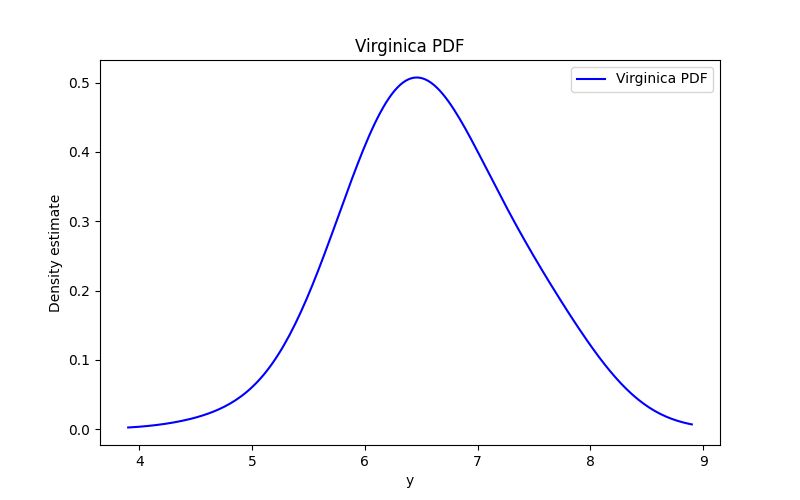
\includegraphics[width=0.8\textwidth]{virginica_pdf.png}
\end{figure}
\begin{figure}[htbp]
    \centering
    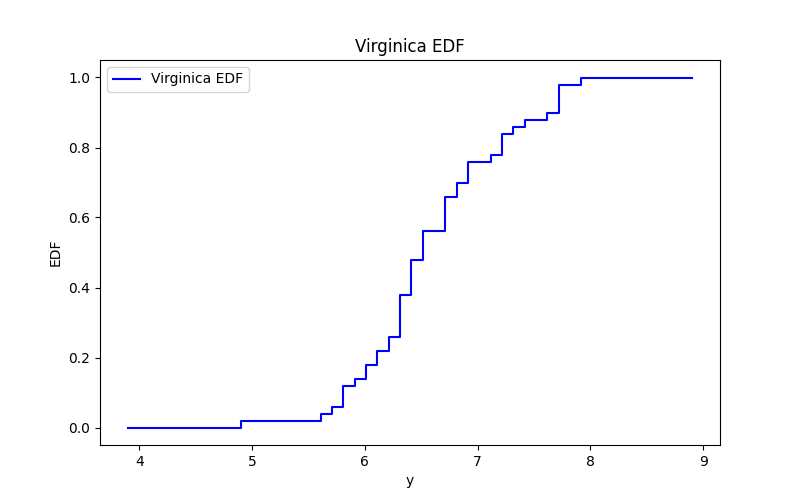
\includegraphics[width=0.8\textwidth]{virginica_edf.png}
\end{figure}
\begin{figure}[htbp]
    \centering
    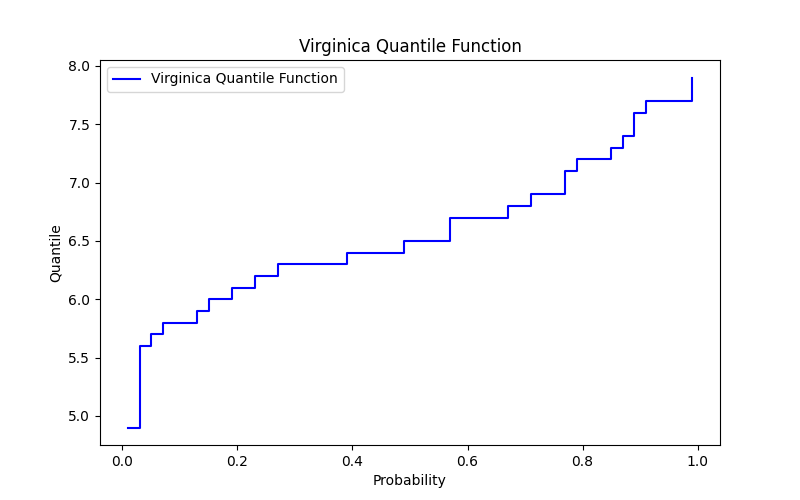
\includegraphics[width=0.8\textwidth]{virginica_quantile.png}
\end{figure}
\newpage
Setosa:
\begin{figure}[htbp]
    \centering
    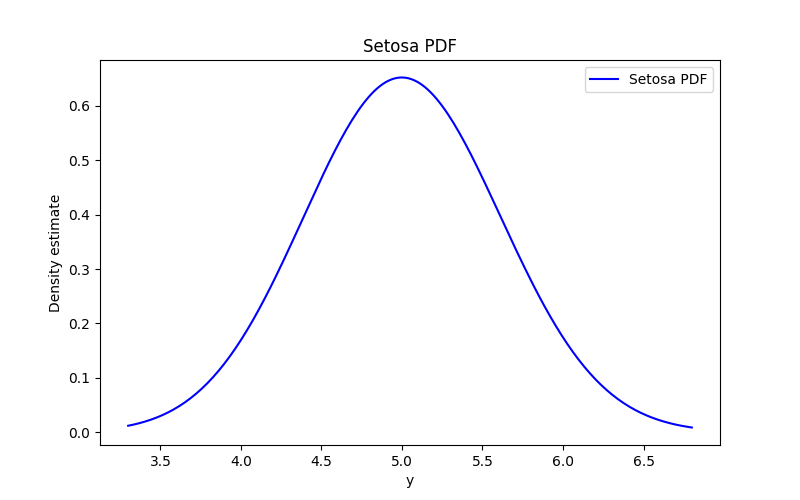
\includegraphics[width=0.8\textwidth]{setosa_pdf.png}
\end{figure}
\begin{figure}[htbp]
    \centering
    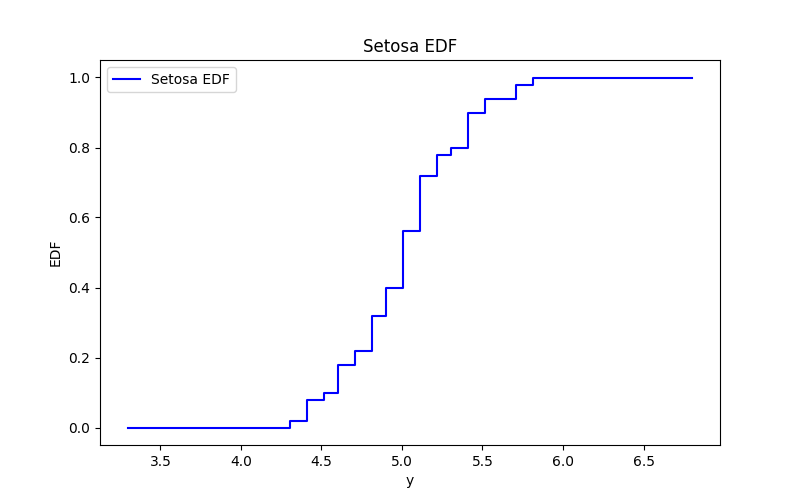
\includegraphics[width=0.8\textwidth]{setosa_edf.png}
\end{figure}
\begin{figure}[htbp]
    \centering
    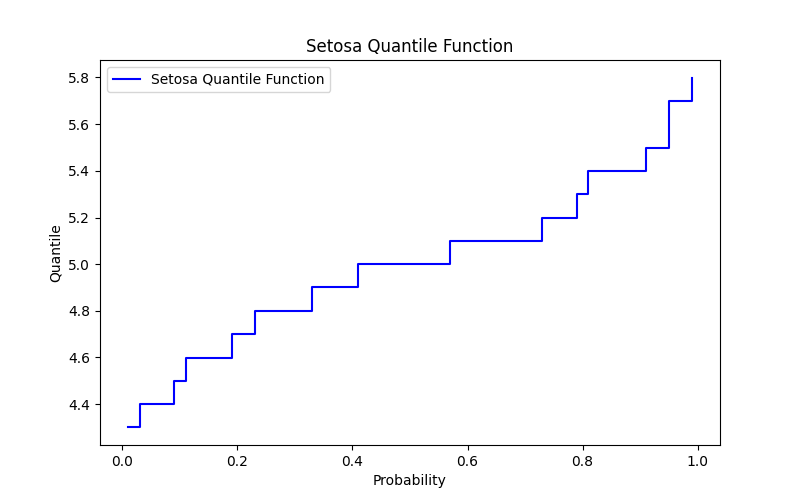
\includegraphics[width=0.8\textwidth]{setosa_quantile.png}
\end{figure}
\newpage 
Generated with the following code: \\
\begin{verbatim}
import math
import numpy as np
import matplotlib.pyplot as plt
def K(u):
    return 1 / math.sqrt(2 * math.pi) * math.e**(-u**2 / 2) 

def kernel_estimator(n, h, kernel_function, data, y):
    result = 0
    coefficient = 1 / (n * h)
    smallest_weight = 10000000
    smallest_weight_y = 0
    largest_weight = 0
    largest_weight_y = 0
    for i in range(0, len(data)):
        input = (y - data[i]) / h
        weight = kernel_function(input)
        if(weight < smallest_weight):
            smallest_weight = weight
            smallest_weight_y = data[i]
        if(weight > largest_weight):
            largest_weight = weight
            largest_weight_y = data[i]
        result += kernel_function(input)
    print("smallest weight: ", smallest_weight, " y: ", smallest_weight_y)
    print("largest weight: ", largest_weight, " y: ", largest_weight_y)
    return coefficient * result

def generate_graphs(data, prefix):
    data = sorted(data)
    n = len(data)
    h = 0.5

    y_values = np.linspace(min(data) - 1, max(data) + 1, 200)
    estimates = [kernel_estimator(n, h, K, data, y) for y in y_values]

    plt.figure(figsize=(8, 5))
    plt.plot(y_values, estimates, label=prefix + ' PDF', color='blue')
    plt.title(prefix + ' PDF')
    plt.xlabel('y')
    plt.ylabel('Density estimate')
    plt.legend()
    plt.show()

    edf_values = [np.sum(data <= y) / n for y in y_values]

    plt.figure(figsize=(8, 5))
    plt.step(y_values, edf_values, where='post', label=prefix + ' EDF', color='blue')
    plt.title(prefix + ' EDF')
    plt.xlabel('y')
    plt.ylabel('EDF')
    plt.legend()
    plt.show()

    n = len(data)

    probs = np.linspace(0, 1, n, endpoint=False) + 1/(2*n)

    plt.figure(figsize=(8, 5))
    plt.step(probs, data, where='post', color='blue', label=prefix + ' Quantile Function')
    plt.title(prefix + ' Quantile Function')
    plt.xlabel('Probability')
    plt.ylabel('Quantile')
    plt.legend()
    plt.show()

if __name__ == "__main__":
    virginica_data = [
        6.3, 5.8, 7.1, 6.3, 6.5, 7.6, 4.9, 7.3, 6.7, 7.2,
        6.5, 6.4, 6.8, 5.7, 5.8, 6.4, 6.5, 7.7, 7.7, 6.0,
        6.9, 5.6, 7.7, 6.3, 6.7, 7.2, 6.2, 6.1, 6.4, 7.2,
        7.4, 7.9, 6.4, 6.3, 6.1, 7.7, 6.3, 6.4, 6.0, 6.9,
        6.7, 6.9, 5.8, 6.8, 6.7, 6.7, 6.3, 6.5, 6.2, 5.9
    ]
    iris_setosa_data = [
        5.1, 4.9, 4.7, 4.6, 5.0, 5.4, 4.6, 5.0, 4.4, 4.9,
        5.4, 4.8, 4.8, 4.3, 5.8, 5.7, 5.4, 5.1, 5.7, 5.1,
        5.4, 5.1, 4.6, 5.1, 4.8, 5.0, 5.0, 5.2, 5.2, 4.7,
        4.8, 5.4, 5.2, 5.5, 4.9, 5.0, 5.5, 4.9, 4.4, 5.1,
        5.0, 4.5, 4.4, 5.0, 5.1, 4.8, 5.1, 4.6, 5.3, 5.0
    ]
    f_5 = kernel_estimator(len(virginica_data), .5, K, virginica_data, 5)
    print("f_5: ", f_5)

    f_7 = kernel_estimator(len(virginica_data), .5, K, virginica_data, 7)
    print("f_7: ", f_7)
    generate_graphs(virginica_data, prefix="Virginica")
    generate_graphs(iris_setosa_data, "Setosa")
\end{verbatim}
\item The distributions appear to be approximately normally distributed.
\end{enumerate}
\section*{Question Group 3}
\begin{enumerate}
\item B \\
\item B \\
\item B \\
\item C \\
\item C \\
\item C \\
\item B \\
\item B \\
\item C \\
\item B \\
\item C
\end{enumerate}
\end{document}